\chapter{Üzembe helyezés és kísérleti eredmények}
\label{chap:uzembehelyezes}

Ebben a fejezetben az elkészült rendszer gyakorlati üzembe helyezését és a végső kísérleti eredményeket mutatom be. A hangsúly itt már nem azon van, hogy milyen komponensekből épül fel a rendszer, hanem azon, hogy a megtervezett feldolgozási folyamat ténylegesen hogyan viselkedik mérés közben. Igyekeztem nem egyetlen jól sikerült futásra támaszkodni, hanem több ismétlésből levonni következtetést, mert kis adathalmaz és neurális háló esetén a véletlen inicializáció és a tanítás lefutása szemmel láthatóan befolyásolja a végeredményt.

A fejezet fő mérései a saját Log-Mel spektrogram alapú 2D CNN modellre vonatkoznak, mert ez adja a dolgozat saját, valós időben használt felismerő pipeline-ját. Kiegészítésként bemutatom a YAMNet alapú transzfer tanulási összehasonlítást is, amely erős előtanított audio reprezentációra épül, de nem váltja ki a saját megoldást.

\section{Üzembe helyezési lépések}
\label{sec:uzembehelyezes}

A valós idejű felismerő alkalmazás a saját, Log-Mel bemenetű 2D CNN modellt használja. Ez fontos különbség a transzfer tanulásos megközelítéssel szemben: a valós idejű demóban nem egy külső, előtanított modell adja a végső felismerést, hanem a dolgozat során felépített saját feldolgozási lánc.

A rendszer futtatásához a következő fő lépések szükségesek:

\begin{enumerate}
    \item \textbf{Python környezet előkészítése.} A projekt futtatásához Python 3.10 vagy újabb verziót használtam, külön virtuális környezettel:
\begin{verbatim}
python3 -m venv venv
source venv/bin/activate
\end{verbatim}

    \item \textbf{Függőségek telepítése.} A szükséges csomagokat a \texttt{requirements.txt} alapján lehet telepíteni:
\begin{verbatim}
pip install -r requirements.txt
\end{verbatim}
    A rendszer főbb könyvtárai a \texttt{tensorflow}, a \texttt{librosa}, a \texttt{numpy}, a \texttt{matplotlib}, valamint a mikrofonos bemenethez használt \texttt{sounddevice}. macOS alatt a \texttt{sounddevice} használatához a PortAudio telepítése is szükséges:
\begin{verbatim}
brew install portaudio
\end{verbatim}

    \item \textbf{A végső modell kiválasztása.} A tanítás során minden futás külön időbélyeges checkpointot hoz létre a \texttt{models/} mappa megfelelő alkönyvtárában. A végső valós idejű futtatáshoz az \texttt{exp\_final} kísérlet validáción legjobb Log-Mel modelljét használtam.

    \item \textbf{Valós idejű felismerő indítása.} A saját modellre épülő valós idejű felismerő az alábbi paranccsal indítható:
\begin{verbatim}
python scripts/05a_realtime_recognition.py
\end{verbatim}
\end{enumerate}

A valós idejű alkalmazásban a bemeneti hang egy 1 másodperces csúszóablakon keresztül kerül feldolgozásra. A modell minden ablakból Log-Mel spektrogramot számol, majd a predikciókat rövid mozgóátlagos simítással stabilizálja. Ez nem javítja meg a modellt statisztikai értelemben, de a felhasználói oldalon sokat számít: a kijelzés kevésbé ugrál, és a bizonytalan pillanatnyi predikciók nem jelennek meg azonnal végleges döntésként.

\section{Kísérleti protokoll}
\label{sec:kiserleti_protokoll}

A mérések célja nem csak az volt, hogy kapjak egy végső pontossági értéket, hanem az is, hogy külön-külön látszódjon az augmentáció, a domain shift és a mikrofonos célkörnyezeti adatok hatása. Emiatt négy kísérleti adathalmazt állítottam össze. Ezek közelítő méretét a \ref{tab:experiment_dataset_sizes}.~táblázat foglalja össze. A táblázatban az osztályonkénti ideális, kerekített mennyiségeket használom, mert a kísérleti felépítés így sokkal könnyebben átlátható.

\begin{table}[H]
\centering
\caption{A négy kísérleti adathalmaz közelítő, osztályonként levezetett mérete}
\label{tab:experiment_dataset_sizes}
\small
\begin{tabular}{lccc}
\toprule
\textbf{Kísérlet} & \textbf{Train} & \textbf{Val} & \textbf{Test} \\
\midrule
Clean baseline & \shortstack{\(7 \times 350\)\\\(\approx 2450\)} & \shortstack{clean\\\(7 \times 75 \approx 525\)} & \shortstack{clean\\\(7 \times 75 \approx 525\)} \\
Augmented & \shortstack{\(7 \times (350 + 350)\)\\\(\approx 4900\)} & \shortstack{clean\\\(7 \times 75 \approx 525\)} & \shortstack{clean\\\(7 \times 75 \approx 525\)} \\
Naive deployment & \shortstack{\(7 \times (350 + 350)\)\\\(\approx 4900\)} & \shortstack{mic\\\(7 \times 75 \approx 525\)} & \shortstack{mic\\\(7 \times 75 \approx 525\)} \\
Final system & \shortstack{\(7 \times (350 + 350 + 350)\)\\\(\approx 7350\)} & \shortstack{mic\\\(7 \times 75 \approx 525\)} & \shortstack{mic\\\(7 \times 75 \approx 525\)} \\
\bottomrule
\end{tabular}
\end{table}

A táblázatban és a \ref{fig:experiment_dataset_distribution}.~ábrán szándékosan kerekített értékeket használok. A kísérleti fázisok logikája így áttekinthetőbb: nem az egyes osztályok néhány mintás eltérése a lényeg, hanem az, hogy egy osztályon belül az eredeti \(70\%-15\%-15\%\)-os felosztás körülbelül \(350\)-\(75\)-\(75\) mintát jelent. A clean baseline a tiszta internetes adatokat adja, az augmented kísérlet a szoftveres augmentáció hatását méri, a naive deployment a mikrofonos validációs/tesztkörnyezetre való átvitel nehézségét mutatja, a final system pedig már a mikrofonos tanítóanyaggal kiegészített végső felállás. Az augmentált és mikrofonos tanítóanyag tehát a train részt növeli, miközben a validációs és teszthalmaz külön marad. Az ábrán a train, validation és test részek külön színcsaládot kaptak, ezeken belül pedig az árnyalat jelzi, hogy clean, augmentált vagy mikrofonos adatról van szó.

\begin{figure}[H]
\centering
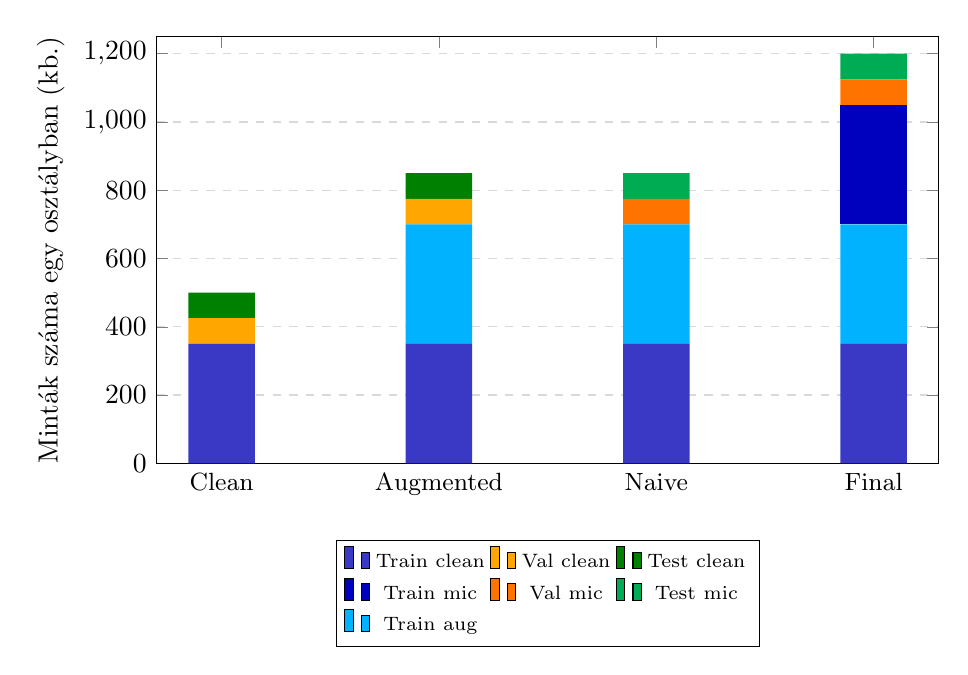
\begin{tikzpicture}
\begin{axis}[
    ybar stacked,
    bar width=24pt,
    width=0.95\textwidth,
    height=7cm,
    ymin=0,
    ymax=1250,
    ylabel={Minták száma egy osztályban (kb.)},
    symbolic x coords={Clean, Augmented, Naive, Final},
    xtick=data,
    x tick label style={font=\small},
    legend style={at={(0.5,-0.18)}, anchor=north, legend columns=3, font=\scriptsize},
    ymajorgrids=true,
    grid style={dashed, gray!30},
]
\addplot[fill=blue!55!gray, draw=none, forget plot] coordinates {
    (Clean,350)
    (Augmented,350)
    (Naive,350)
    (Final,350)
};
\addplot[fill=blue!30!cyan, draw=none, forget plot] coordinates {
    (Clean,0)
    (Augmented,350)
    (Naive,350)
    (Final,350)
};
\addplot[fill=blue!75!black, draw=none, forget plot] coordinates {
    (Clean,0)
    (Augmented,0)
    (Naive,0)
    (Final,350)
};
\addplot[fill=orange!70!yellow, draw=none, forget plot] coordinates {
    (Clean,75)
    (Augmented,75)
    (Naive,0)
    (Final,0)
};
\addplot[fill=orange!90!red, draw=none, forget plot] coordinates {
    (Clean,0)
    (Augmented,0)
    (Naive,75)
    (Final,75)
};
\addplot[fill=green!50!black, draw=none, forget plot] coordinates {
    (Clean,75)
    (Augmented,75)
    (Naive,0)
    (Final,0)
};
\addplot[fill=green!35!teal, draw=none, forget plot] coordinates {
    (Clean,0)
    (Augmented,0)
    (Naive,75)
    (Final,75)
};
\addlegendimage{ybar, ybar legend, fill=blue!55!gray, draw=none}
\addlegendentry{Train clean}
\addlegendimage{ybar, ybar legend, fill=orange!70!yellow, draw=none}
\addlegendentry{Val clean}
\addlegendimage{ybar, ybar legend, fill=green!50!black, draw=none}
\addlegendentry{Test clean}
\addlegendimage{ybar, ybar legend, fill=blue!75!black, draw=none}
\addlegendentry{Train mic}
\addlegendimage{ybar, ybar legend, fill=orange!90!red, draw=none}
\addlegendentry{Val mic}
\addlegendimage{ybar, ybar legend, fill=green!35!teal, draw=none}
\addlegendentry{Test mic}
\addlegendimage{ybar, ybar legend, fill=blue!30!cyan, draw=none}
\addlegendentry{Train aug}
\end{axis}
\end{tikzpicture}
\caption{A kísérleti adathalmazok közelítő megoszlása egy átlagos osztályra vetítve}
\label{fig:experiment_dataset_distribution}
\end{figure}

A modellválasztást minden kísérletnél a validációs halmazon végeztem. Minden kísérletet ötször futtattam le egymás után, majd az eredményeket átlag és szórás formájában összesítettem. Erre azért volt szükség, mert a kis méretű adathalmaz és a neurális háló sztochasztikus tanítása miatt egyetlen futás eredménye nem adna elég stabil képet. A végső teszthalmazt csak a modellválasztás után, egyszer használtam: az \texttt{exp\_final} kísérlet legjobb validációs Macro F1 értékű checkpointját töltöttem vissza, és azt futtattam le a test halmazon.

A kísérletek során két fő mérőszámot használtam:
\begin{itemize}
    \item \textbf{Accuracy:} az összes mintára vetített találati arány.
    \item \textbf{Macro F1:} az osztályonként számolt F1-score-ok egyszerű átlaga, amely jobban megmutatja, ha a modell bizonyos osztályokat elhanyagol.
\end{itemize}

Hangszerfelismerésnél a Macro F1 különösen fontos, mert nem elég az, hogy a modell összességében sok mintát eltaláljon. Az is lényeges, hogy a gitár, zongora, vokál, vonós, nád- és rézfúvós, valamint zaj osztályok között ne legyen túl nagy teljesítménybeli különbség.

\section{A bemeneti reprezentáció kiválasztása a clean baseline alapján}
\label{sec:feature_valasztas}

Mielőtt a négy kísérleti fázist végigfuttattam volna, külön meg kellett indokolni, hogy a saját CNN modell milyen bemeneti reprezentációval dolgozzon tovább. A rendszer tervezési részében három jellegzetes jellemzőkinyerési módszert vizsgáltam: MFCC-t, STFT spektrogramot és Log-Mel spektrogramot. Ezek közül nem elméleti alapon választottam ki egyet, hanem a clean baseline adathalmazon mindhárom változatot ötször lefuttattam ugyanazzal a 2D CNN architektúrával.

Ez a mérés azért került a tiszta baseline-ra, mert itt még nincs jelen az augmentáció vagy a mikrofonos domain shift hatása. Így a különbség elsősorban azt mutatja meg, hogy az adott reprezentáció mennyire használható a saját modell számára ideálisabb, tisztább bemenet mellett. A teszthalmazt ebben a lépésben sem használtam: a választás kizárólag validációs eredmények alapján történt.

\begin{table}[H]
\centering
\caption{Jellemzőkinyerési módszerek összehasonlítása a clean baseline validációs futásain}
\label{tab:feature_selection_clean}
\begin{tabular}{lcc}
\toprule
\textbf{Bemeneti reprezentáció} & \textbf{Accuracy} & \textbf{Macro F1} \\
\midrule
MFCC & \(56{,}7 \pm 4{,}6\%\) & \(57{,}0 \pm 5{,}0\%\) \\
STFT & \(61{,}8 \pm 5{,}9\%\) & \(61{,}3 \pm 6{,}1\%\) \\
Log-Mel & \(\mathbf{67{,}7 \pm 6{,}2\%}\) & \(\mathbf{67{,}8 \pm 6{,}3\%}\) \\
\bottomrule
\end{tabular}
\end{table}

\begin{figure}[H]
\centering
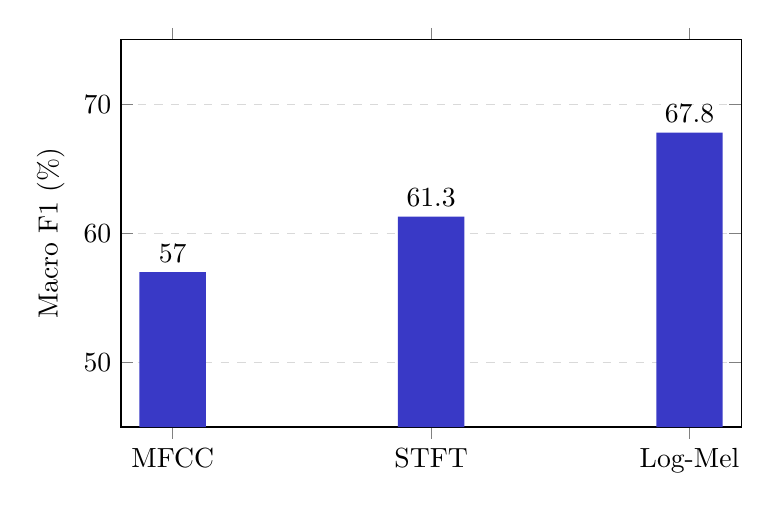
\begin{tikzpicture}
\begin{axis}[
    ybar,
    bar width=24pt,
    width=0.78\textwidth,
    height=6.5cm,
    ymin=45,
    ymax=75,
    ylabel={Macro F1 (\%)},
    symbolic x coords={MFCC, STFT, Log-Mel},
    xtick=data,
    nodes near coords,
    nodes near coords align={vertical},
    ymajorgrids=true,
    grid style={dashed, gray!30},
]
\addplot[fill=blue!55!gray, draw=none] coordinates {
    (MFCC,57.0)
    (STFT,61.3)
    (Log-Mel,67.8)
};
\end{axis}
\end{tikzpicture}
\caption{A clean baseline validációs Macro F1 értékei a három bemeneti reprezentáció esetén}
\label{fig:feature_selection_clean}
\end{figure}

A \ref{tab:feature_selection_clean}.~táblázat és a \ref{fig:feature_selection_clean}.~ábra alapján a Log-Mel spektrogram adta a legerősebb kiindulópontot. Az MFCC a leggyengébb eredményt hozta, ami érthető: bár tömör és klasszikusan jól használható reprezentáció, a DCT lépés miatt olyan finom spektrális részleteket is elveszíthet, amelyek egy CNN számára hasznosak lennének. Az STFT ennél jobb volt, mert több nyers frekvenciainformációt őriz meg, viszont a lineáris frekvenciatengely miatt nagyobb és kevésbé hallásközeli bemenetet ad.

A Log-Mel ezzel szemben jó kompromisszumnak bizonyult. Megőrzi a képszerű idő-frekvencia szerkezetet, amelyet a 2D CNN ki tud használni, miközben a Mel-skála az emberi hallás szempontjából fontosabb tartományokat hangsúlyosabban kezeli. Emiatt a további kísérleti fázisokat -- augmentáció, naive deployment és final system -- már Log-Mel bemenettel futtattam. Ezzel a döntéssel a későbbi összehasonlításokban nem egyszerre változik a reprezentáció és az adathalmaz, hanem a bemenet rögzített marad, és tisztábban láthatóvá válik az adatok összetételének hatása.

\section{Validációs eredmények}
\label{sec:validacios_eredmenyek}

Az öt-öt validációs futás összesítését a \ref{tab:validation_summary}.~táblázat mutatja. Innentől kezdve minden saját CNN kísérleti fázis a kiválasztott Log-Mel reprezentációval futott. A számok alapján jól látszik, hogy a különböző kísérleti fázisok nem csak abszolút pontosságban, hanem stabilitásban is eltérnek egymástól.

\begin{table}[H]
\centering
\caption{Validációs eredmények öt futás alapján}
\label{tab:validation_summary}
\begin{tabular}{lcc}
\toprule
\textbf{Kísérlet} & \textbf{Accuracy} & \textbf{Macro F1} \\
\midrule
Clean baseline & \(67{,}7 \pm 6{,}2\%\) & \(67{,}8 \pm 6{,}3\%\) \\
Augmented & \(79{,}2 \pm 2{,}2\%\) & \(79{,}2 \pm 2{,}2\%\) \\
Naive deployment & \(67{,}3 \pm 3{,}6\%\) & \(67{,}2 \pm 3{,}9\%\) \\
Final system & \(76{,}9 \pm 1{,}8\%\) & \(76{,}8 \pm 2{,}1\%\) \\
\bottomrule
\end{tabular}
\end{table}

A \ref{fig:macro_f1_trend}.~ábra ugyanezt a folyamatot vizuálisan mutatja. Az ábra nem egyetlen futás szerencséjét ábrázolja, hanem az öt futás átlagos Macro F1 értékét.

\begin{figure}[H]
\centering
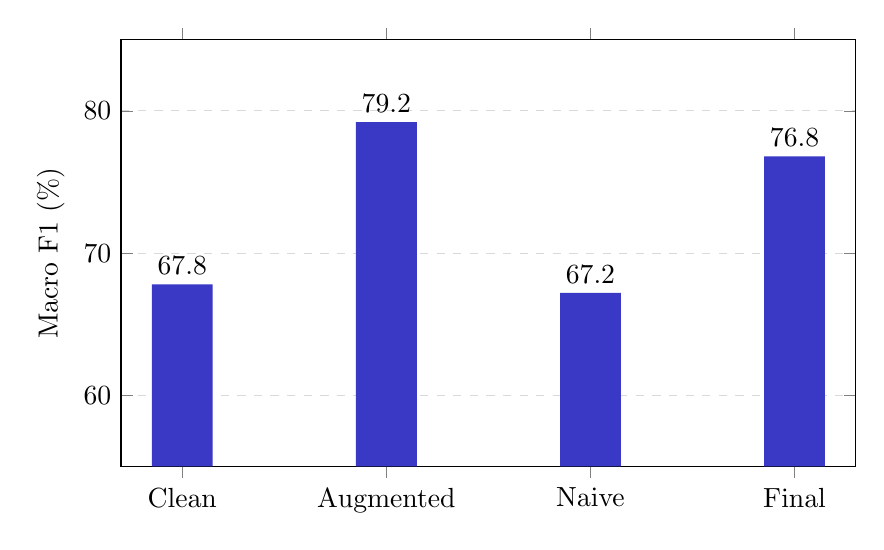
\begin{tikzpicture}
\begin{axis}[
    ybar,
    bar width=22pt,
    width=0.9\textwidth,
    height=7cm,
    ymin=55,
    ymax=85,
    ylabel={Macro F1 (\%)},
    symbolic x coords={Clean, Augmented, Naive, Final},
    xtick=data,
    nodes near coords,
    nodes near coords align={vertical},
    ymajorgrids=true,
    grid style={dashed, gray!30},
]
\addplot[fill=blue!55!gray, draw=none] coordinates {
    (Clean,67.8)
    (Augmented,79.2)
    (Naive,67.2)
    (Final,76.8)
};
\end{axis}
\end{tikzpicture}
\caption{A validációs Macro F1 értékek alakulása a négy kísérleti fázisban}
\label{fig:macro_f1_trend}
\end{figure}

Az eredmények alapján az augmentáció hatása egyértelműen pozitív. A tiszta baseline \(67{,}8\%\)-os Macro F1 értékéhez képest az augmentált kísérlet \(79{,}2\%\)-ot ért el. Ez azt jelenti, hogy a mesterségesen hozzáadott torzítások, zajok és szobaszerű visszaverődések nem csak több adatot adtak a modellnek, hanem valóban segítették az általánosabban használható mintázatok megtanulását.

A naive deployment kísérlet ezzel szemben visszaesett \(67{,}2\%\)-os Macro F1 értékre. Ez a mérés számomra a dolgozat egyik legfontosabb tanulsága: ha a modellt tiszta és szoftveresen augmentált adatokon tanítjuk, majd mikrofonos környezetben próbáljuk használni, a domain shift mérhető teljesítményromlást okoz. Más szóval a valós idejű működéshez nem elég a letöltött vagy tisztított hanganyag, mert a konkrét mikrofon, hangszóró, szoba és zajprofil is beleszól abba, mit lát a modell.

A final system kísérletben a mikrofonos train adatok is bekerültek a tanításba. Ennek hatására a Macro F1 \(76{,}8\%\)-ra emelkedett, vagyis a rendszer a naiv mikrofonos kiértékeléshez képest a teljesítmény nagy részét visszanyerte. Ez nem azt jelenti, hogy a modell hibátlan lett, de mérnöki szempontból jól látható, hogy a célkörnyezeti adatok bevonása működő domain adaptation lépésnek bizonyult.

\begin{figure}[H]
    \centering
    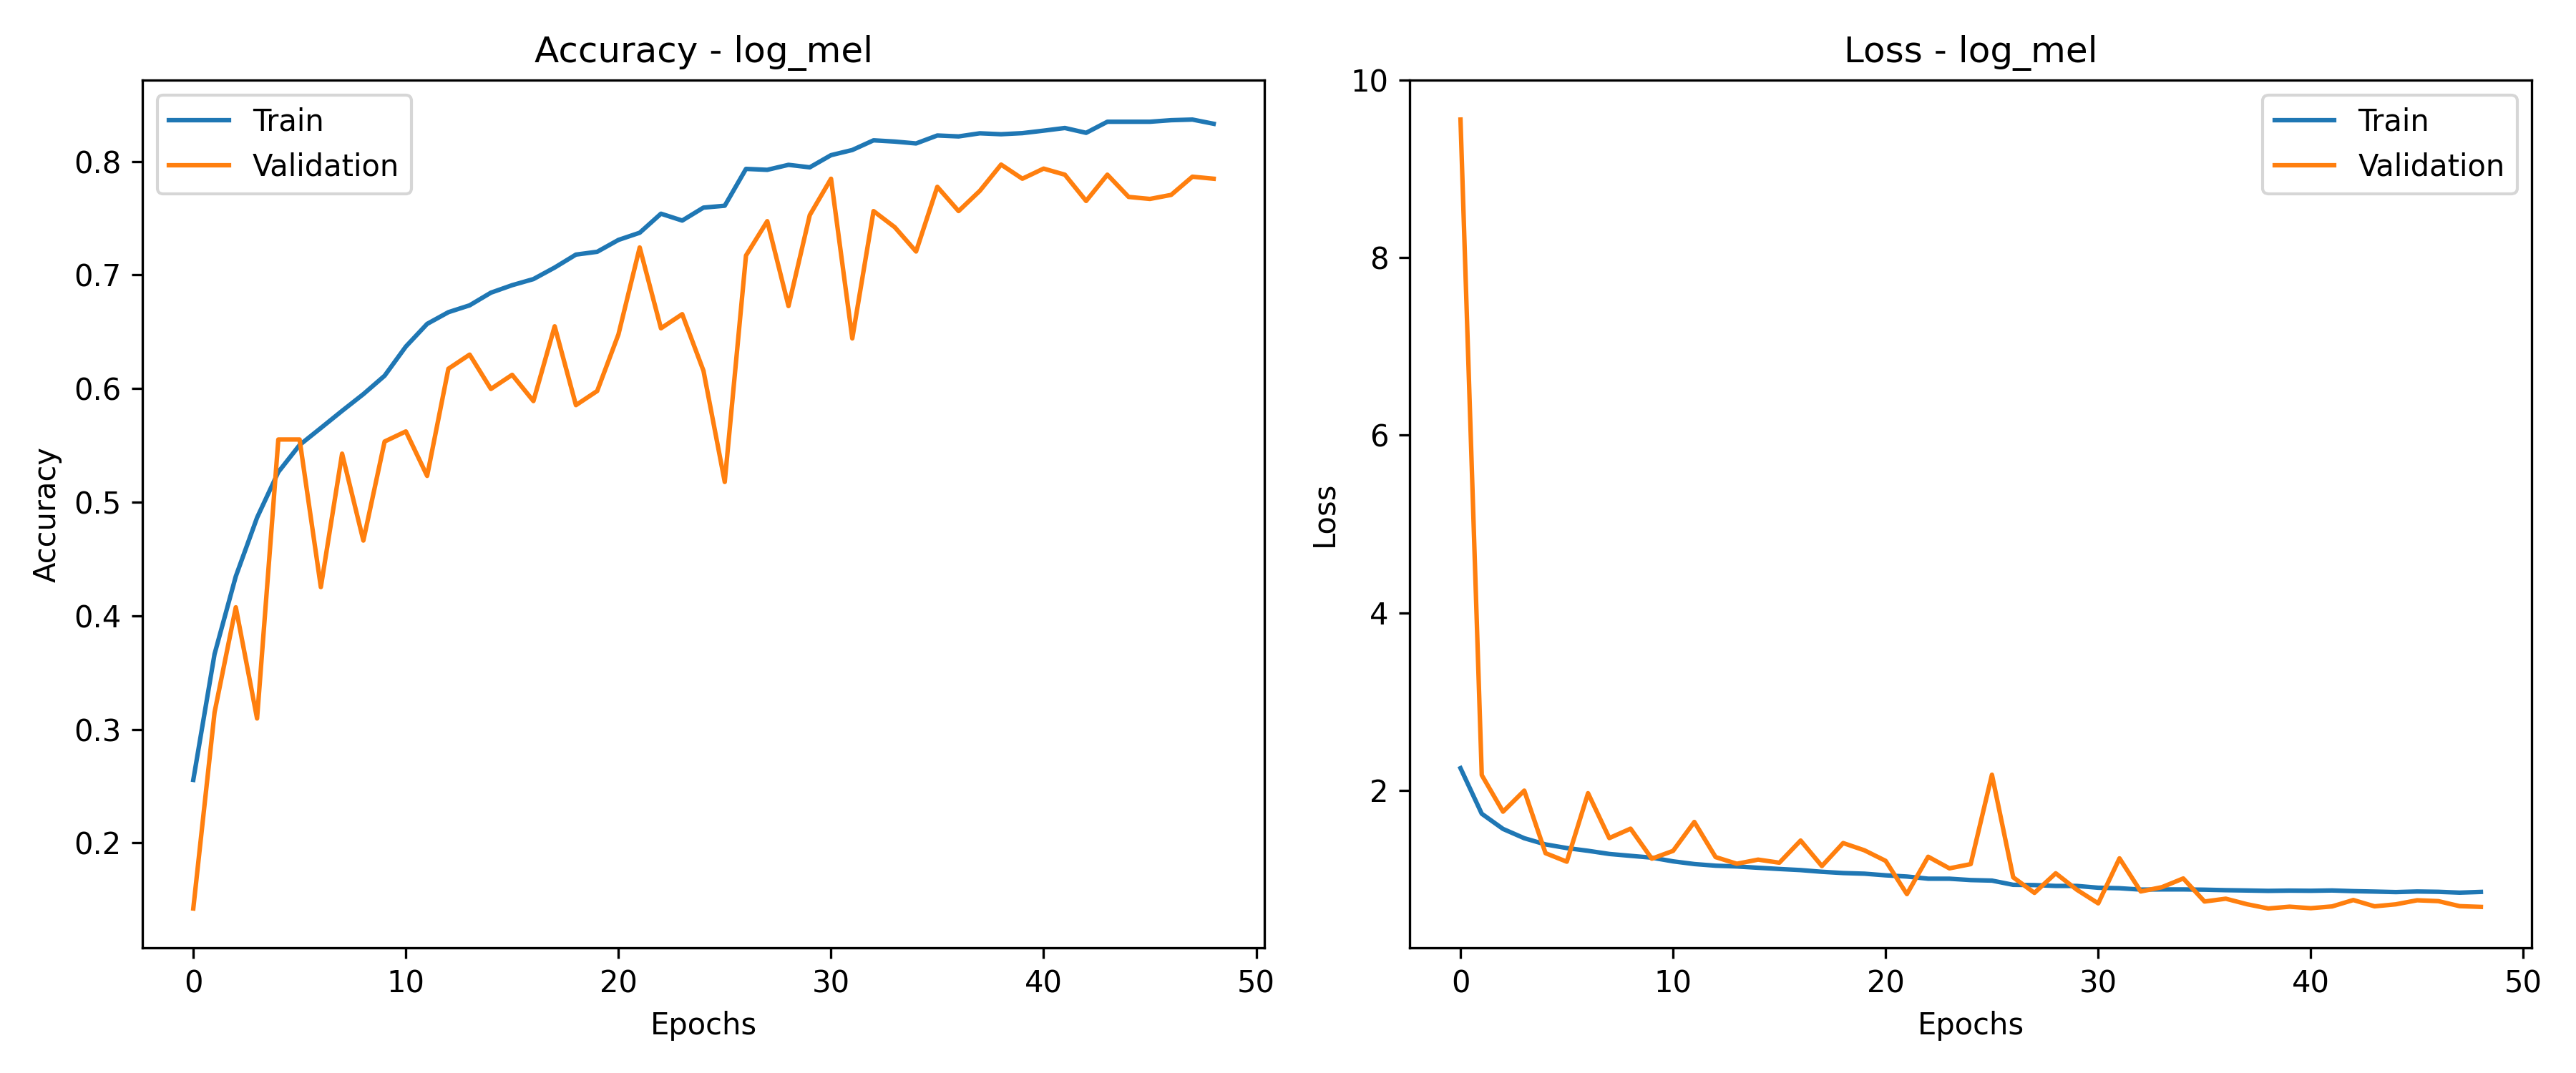
\includegraphics[width=0.9\textwidth]{fig_final_val_learning_curves.png}
    \caption{A legjobb validációs \texttt{exp\_final} futás tanulási görbéi}
    \label{fig:final_val_learning_curves}
\end{figure}

A \ref{fig:final_val_learning_curves}.~ábrán látható tanulási görbék alapján a modell tanítása nem teljesen sima folyamat. Ez várható is: a validációs halmaz néhány száz mintából áll, a bemenetek pedig valós hangmintákból és mikrofonos újrafelvételekből származnak. A görbék emiatt helyenként ugrálnak, viszont a tendencia mégis értelmezhető: a tanítás előrehaladtával a validációs teljesítmény javul, majd egy pont után már nem hoz stabil további nyereséget. Emiatt használtam early stoppingot és a validációs veszteség alapján mentett checkpointot.

\section{Végső teszteredmények}
\label{sec:vegso_teszt}

A végső tesztet már nem használtam modellválasztásra. Először a saját Log-Mel alapú 2D CNN-t értékeltem ki. Az öt \texttt{exp\_final} validációs futás közül a legjobb Macro F1 értékű checkpointot választottam ki:

\begin{center}
\texttt{exp\_final\_log\_mel\_2dcnn\_val\_20260527\_222650\_best\_model.keras}
\end{center}

Ezt a modellt újratanítás nélkül töltöttem vissza, és egyszer futtattam le a félretett teszthalmazon. A végső eredmény:

\begin{center}
\textbf{Accuracy: \(73{,}4\%\), Macro F1: \(72{,}7\%\)}
\end{center}

A részletes osztályonkénti eredményeket a \ref{tab:final_test_report}.~táblázat mutatja.

\begin{table}[H]
\centering
\caption{A végső \texttt{exp\_final} modell teszteredménye osztályonként}
\label{tab:final_test_report}
\begin{tabular}{lrrrr}
\toprule
\textbf{Osztály} & \textbf{Precision} & \textbf{Recall} & \textbf{F1-score} & \textbf{Mintaszám} \\
\midrule
Gitár & 88,5\% & 59,0\% & 70,8\% & 78 \\
Zongora & 75,3\% & 93,6\% & 83,4\% & 78 \\
Vokál & 72,1\% & 79,5\% & 75,6\% & 78 \\
Vonós & 63,0\% & 59,0\% & 60,9\% & 78 \\
Nádfúvós & 64,6\% & 77,1\% & 70,3\% & 83 \\
Rézfúvós & 80,8\% & 50,6\% & 62,2\% & 83 \\
Zaj & 77,6\% & 96,2\% & 85,9\% & 79 \\
\midrule
\textbf{Összesen / átlag} & 75,0\% & 73,4\% & 72,7\% & 557 \\
\bottomrule
\end{tabular}
\end{table}

A teszteredmény reálisabb képet ad a rendszer generalizációjáról, mint a legjobb validációs futás. A validáción elért \(79{,}7\%\)-os Macro F1 a modellválasztáshoz hasznos volt, de a félretett teszthalmazon már \(72{,}7\%\)-os Macro F1 jelent meg. Ezt nem tekintem hibának, inkább fontos figyelmeztetésnek: kis saját adathalmaznál a validációs eredmény optimistább lehet, ezért a végső testmérés nélkül könnyű lenne túlértékelni a rendszert.

\begin{figure}[H]
    \centering
    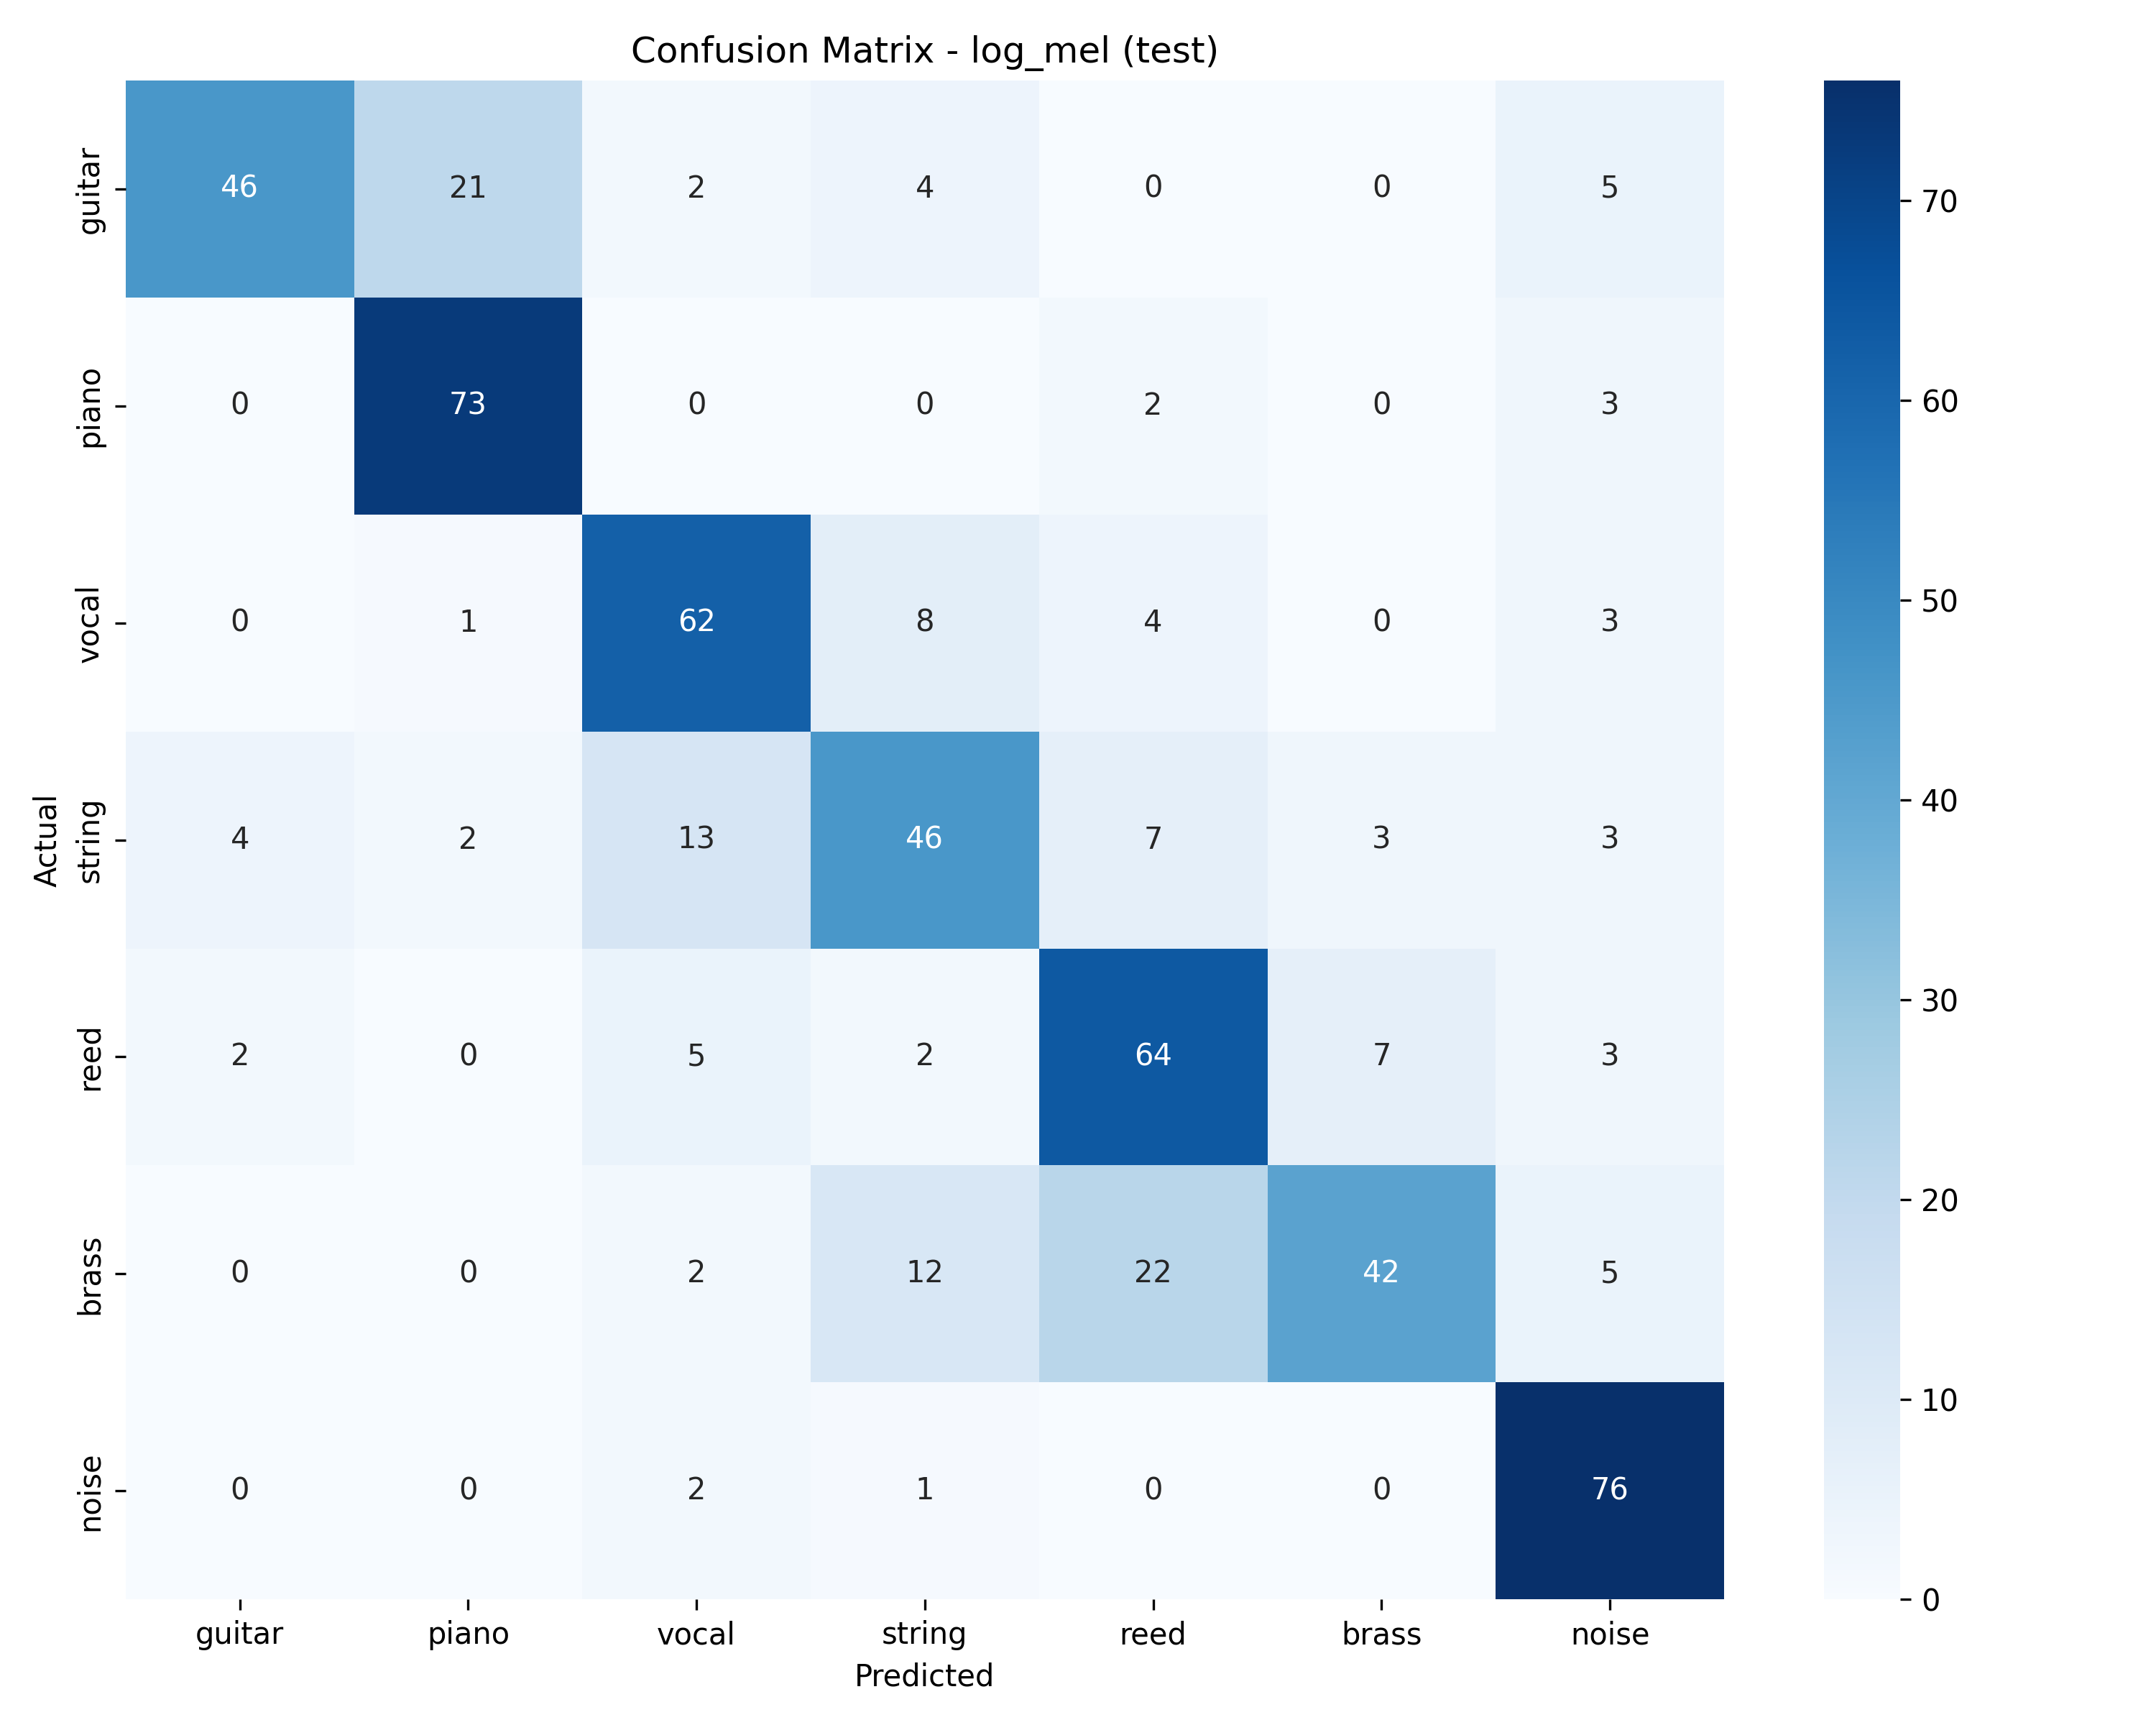
\includegraphics[width=0.82\textwidth]{fig_final_test_confusion_matrix.png}
    \caption{A végső \texttt{exp\_final} modell konfúziós mátrixa a teszthalmazon}
    \label{fig:final_test_confusion_matrix}
\end{figure}

\begin{figure}[H]
    \centering
    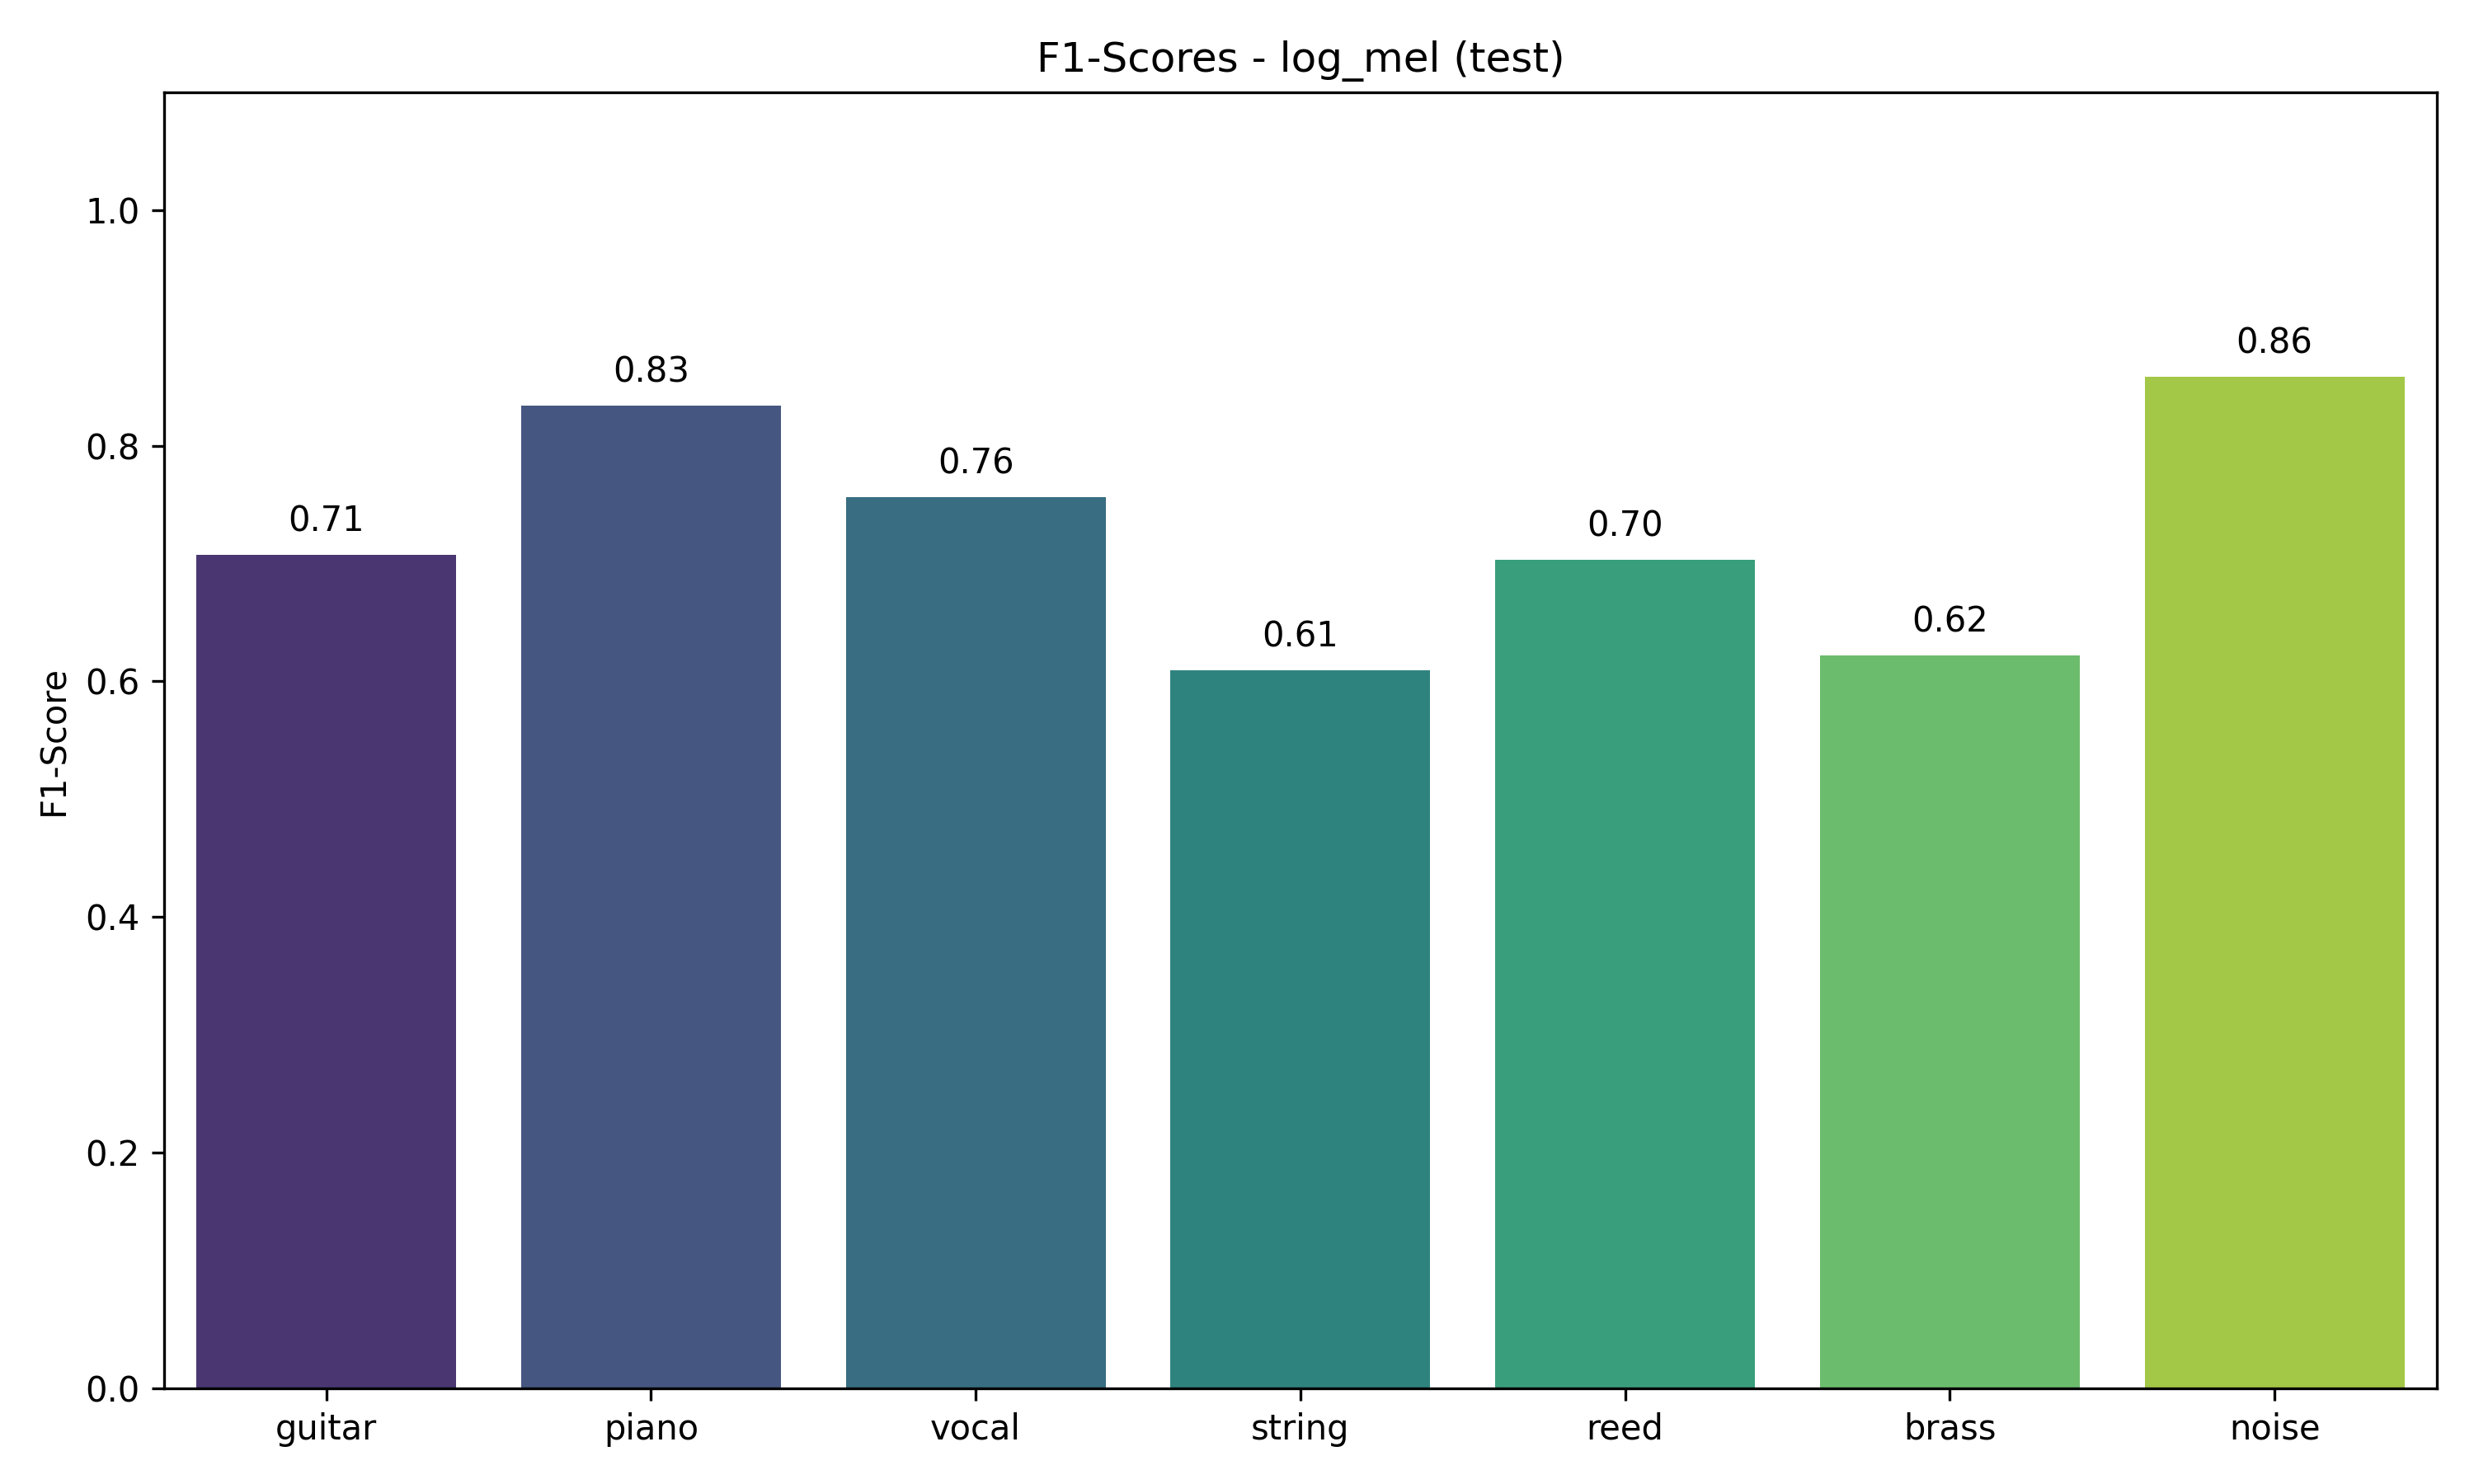
\includegraphics[width=0.82\textwidth]{fig_final_test_f1_scores.png}
    \caption{A végső \texttt{exp\_final} modell osztályonkénti F1-score értékei}
    \label{fig:final_test_f1_scores}
\end{figure}

A \ref{fig:final_test_confusion_matrix}.~ábra alapján a legerősebb osztály a zaj, amely \(85{,}9\%\)-os F1-score-t ért el. Ez gyakorlati szempontból kedvező, mert a valós idejű alkalmazásnak nemcsak hangszert kell felismernie, hanem azt is kezelnie kell, amikor nincs értelmezhető hangszeres bemenet. A zongora szintén erős eredményt adott \(83{,}4\%\)-os F1-score-ral, ami valószínűleg a jellegzetes tranzienseknek és a jól elkülönülő spektrális mintázatnak köszönhető.

A gyengébb pontok főleg a vonós és rézfúvós osztályoknál jelentkeztek. A rézfúvós osztály recall értéke csak \(50{,}6\%\), vagyis a valódi rézfúvós minták közel fele más osztályba került. A konfúziós mátrix szerint ezek jelentős része nádfúvós vagy vonós osztályként jelent meg. Ez akusztikailag nem teljesen meglepő: egyes rézfúvós és nádfúvós hangok felhangszerkezete, megszólalási karaktere és a mikrofonos torzítás miatt látható Log-Mel mintázata közel kerülhet egymáshoz.

A gitár esetében magas precision, de alacsonyabb recall figyelhető meg. Ez azt jelenti, hogy amikor a modell gitárt mond, akkor többnyire igaza van, viszont sok valódi gitármintát nem mer gitárként azonosítani. A hibák egy része zongora irányba megy, ami a pengetett és leütött húrok kezdeti tranziensének hasonlósága miatt értelmezhető.

\subsection{YAMNet transfer learning összehasonlítás}
\label{subsec:yamnet_test}

A saját modell mellett lefuttattam a YAMNet alapú transzfer tanulási változatot is. Ennél a YAMNet befagyasztott előtanított hálóként működik: a nyers 1 másodperces audiojelből 1024 dimenziós embeddinget készít, és csak az erre épített kisebb osztályozófejet tanítom a saját hangszerosztályokra. A validációs futás \(83{,}6\%\)-os accuracy-t és \(83{,}7\%\)-os Macro F1 értéket adott, a kiválasztott checkpoint egyszeri tesztfuttatása pedig a következő eredményt hozta:

\begin{center}
\textbf{YAMNet transfer learning -- Accuracy: \(78{,}8\%\), Macro F1: \(79{,}1\%\)}
\end{center}

\begin{table}[H]
\centering
\caption{A saját Log-Mel modell és a YAMNet transfer learning teszteredményeinek összehasonlítása}
\label{tab:logmel_yamnet_test_comparison}
\begin{tabular}{lcc}
\toprule
\textbf{Modell} & \textbf{Accuracy} & \textbf{Macro F1} \\
\midrule
Saját Log-Mel + 2D CNN & 73,4\% & 72,7\% \\
YAMNet transfer learning & 78,8\% & 79,1\% \\
\bottomrule
\end{tabular}
\end{table}

A YAMNet tehát nem csak minimálisan, hanem mérhetően jobb eredményt adott: körülbelül \(5{,}4\) százalékponttal magasabb accuracy-t és \(6{,}4\) százalékponttal magasabb Macro F1 értéket ért el. Ugyanakkor ez nem nagyságrendi különbség. Ennek több oka is van: a teszthalmaz mikrofonos domainből származik, a hangszerosztályok több konkrét hangszert vonnak össze egy-egy kategóriába, az 1 másodperces minták sokszor csak rövid részletet tartalmaznak, a YAMNet pedig általános AudioSet-feladatokra előtanított modell, nem kifejezetten erre a hét osztályra készült.

Osztályszinten a YAMNet főleg a gitár, vokál és vonós kategóriákon javított sokat. A zaj osztálynál viszont a saját Log-Mel modell maradt erősebb, ami arra utal, hogy a saját pipeline a konkrét zajküszöbölési és mikrofonos környezethez bizonyos szempontból jobban illeszkedett.

\begin{figure}[H]
    \centering
    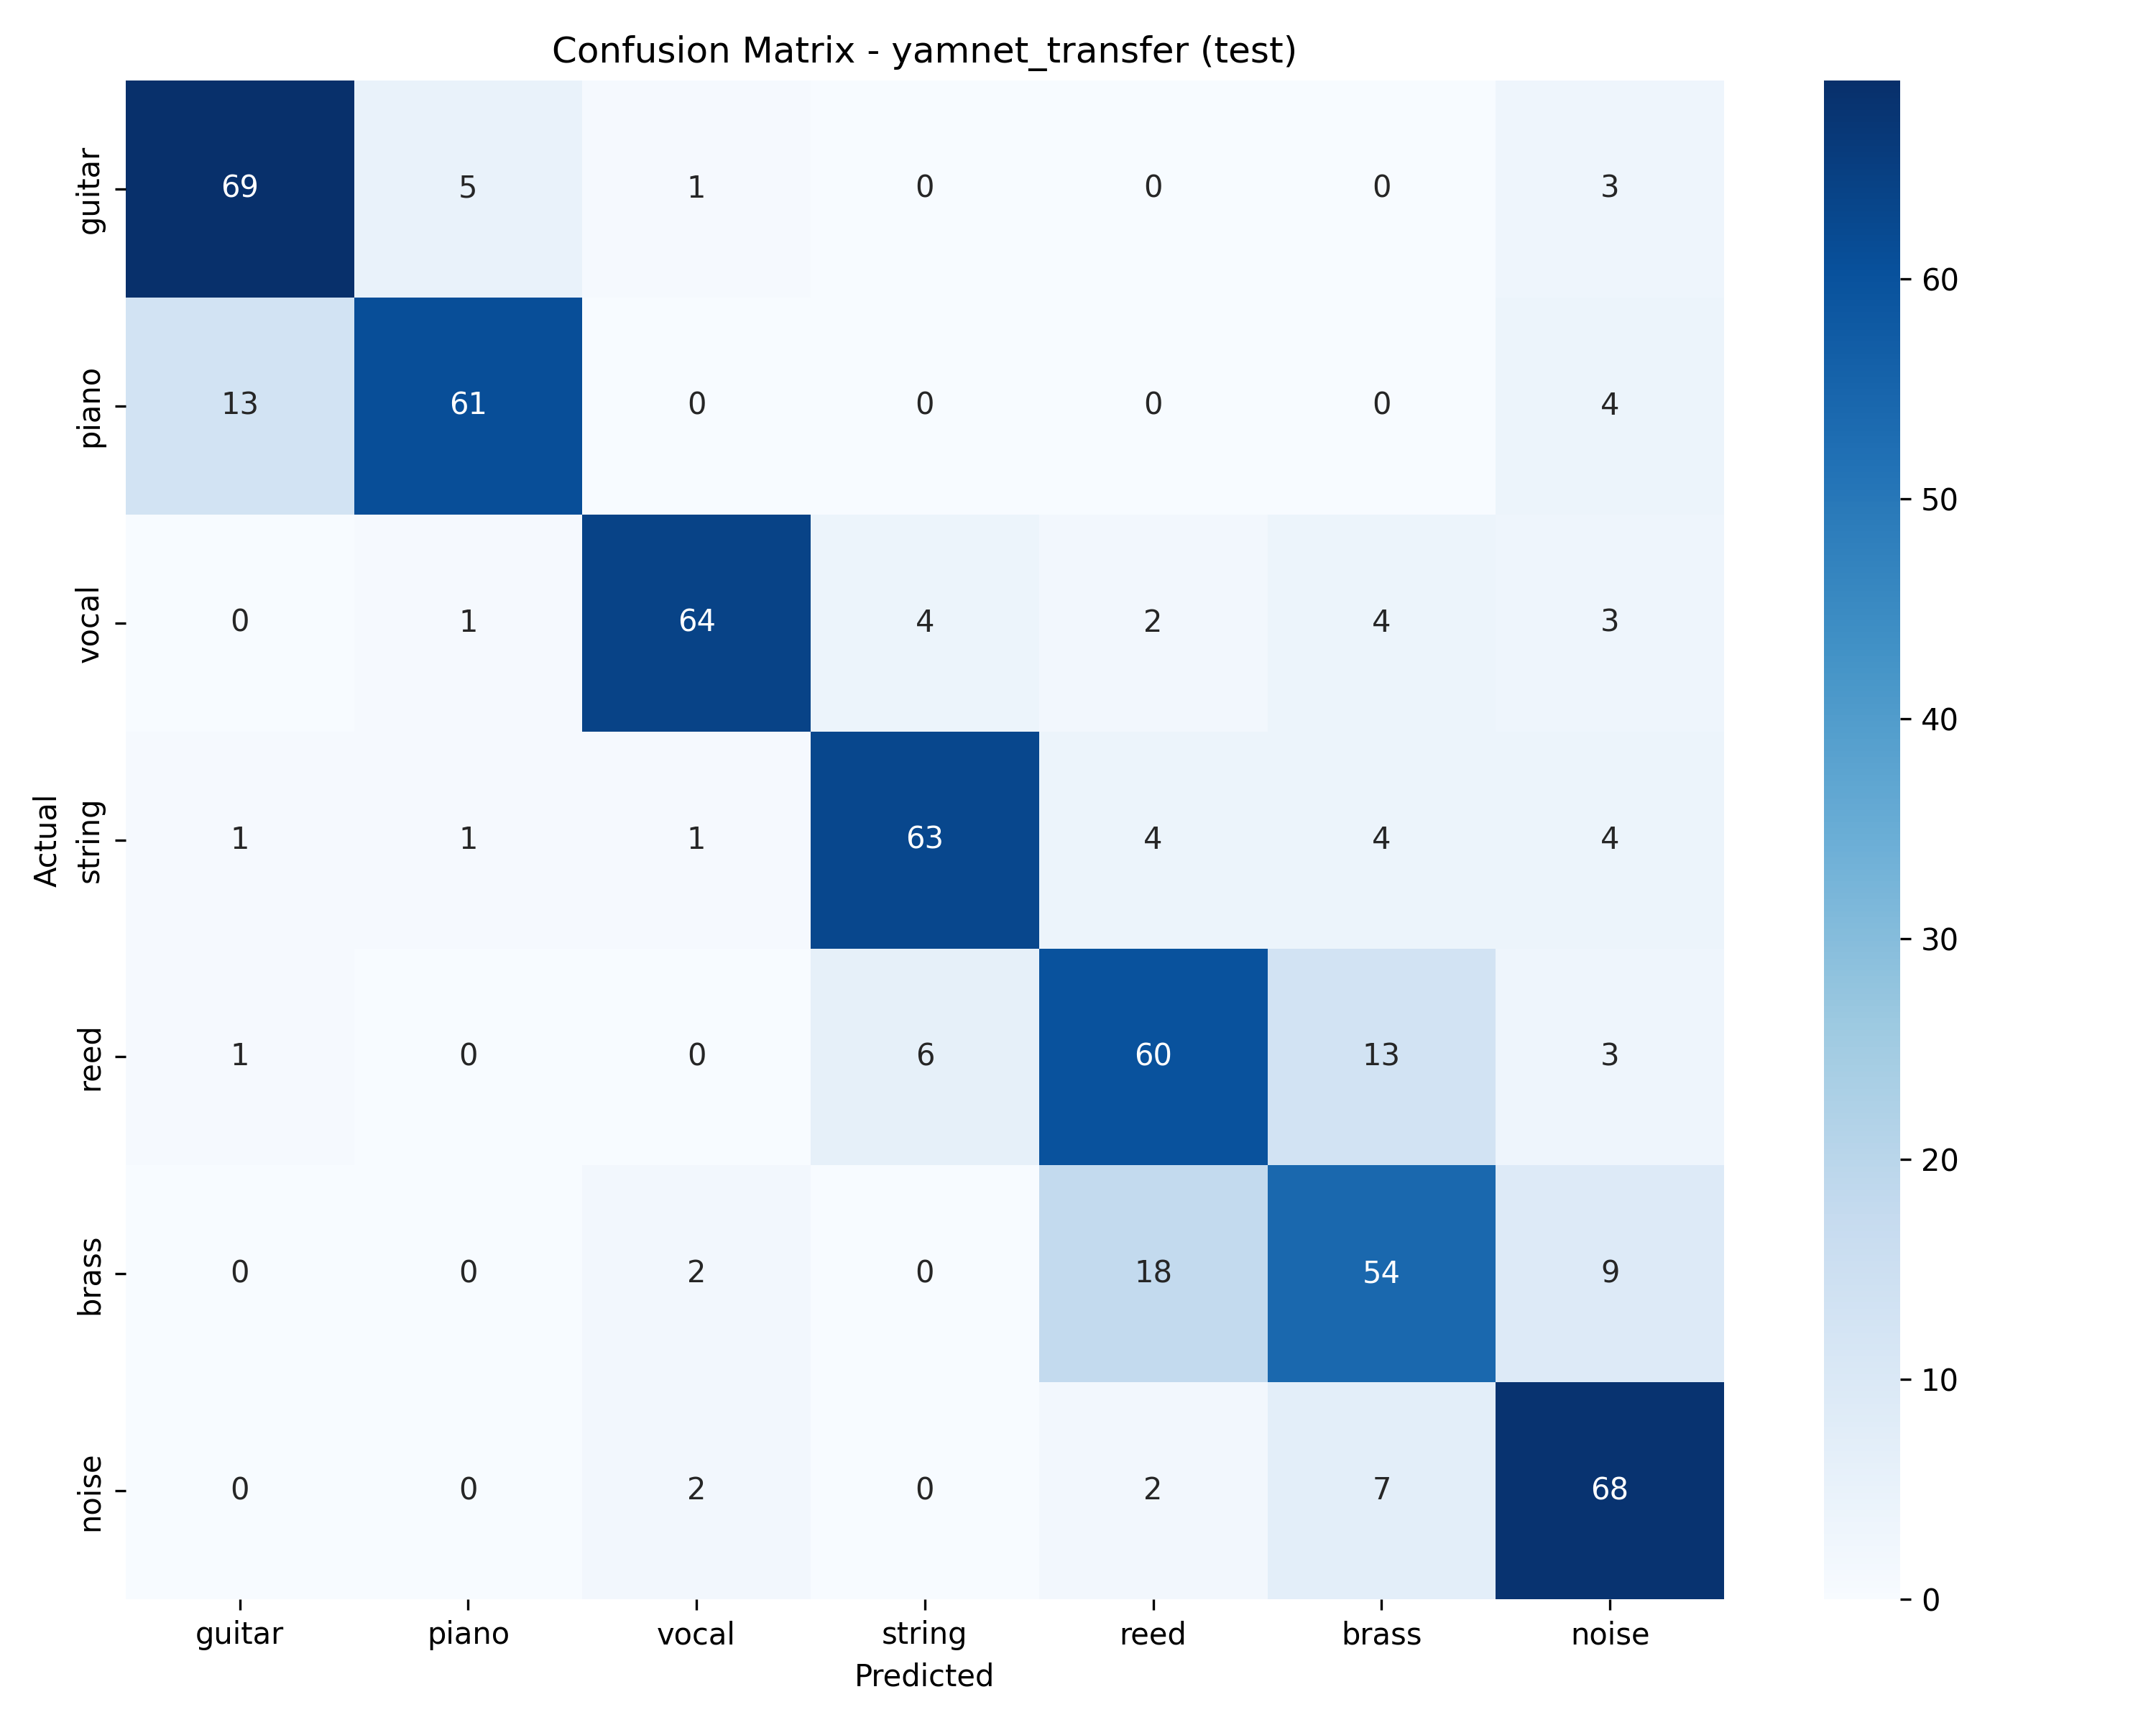
\includegraphics[width=0.82\textwidth]{fig_yamnet_test_confusion_matrix.png}
    \caption{A YAMNet transfer learning modell konfúziós mátrixa a teszthalmazon}
    \label{fig:yamnet_test_confusion_matrix}
\end{figure}

\begin{figure}[H]
    \centering
    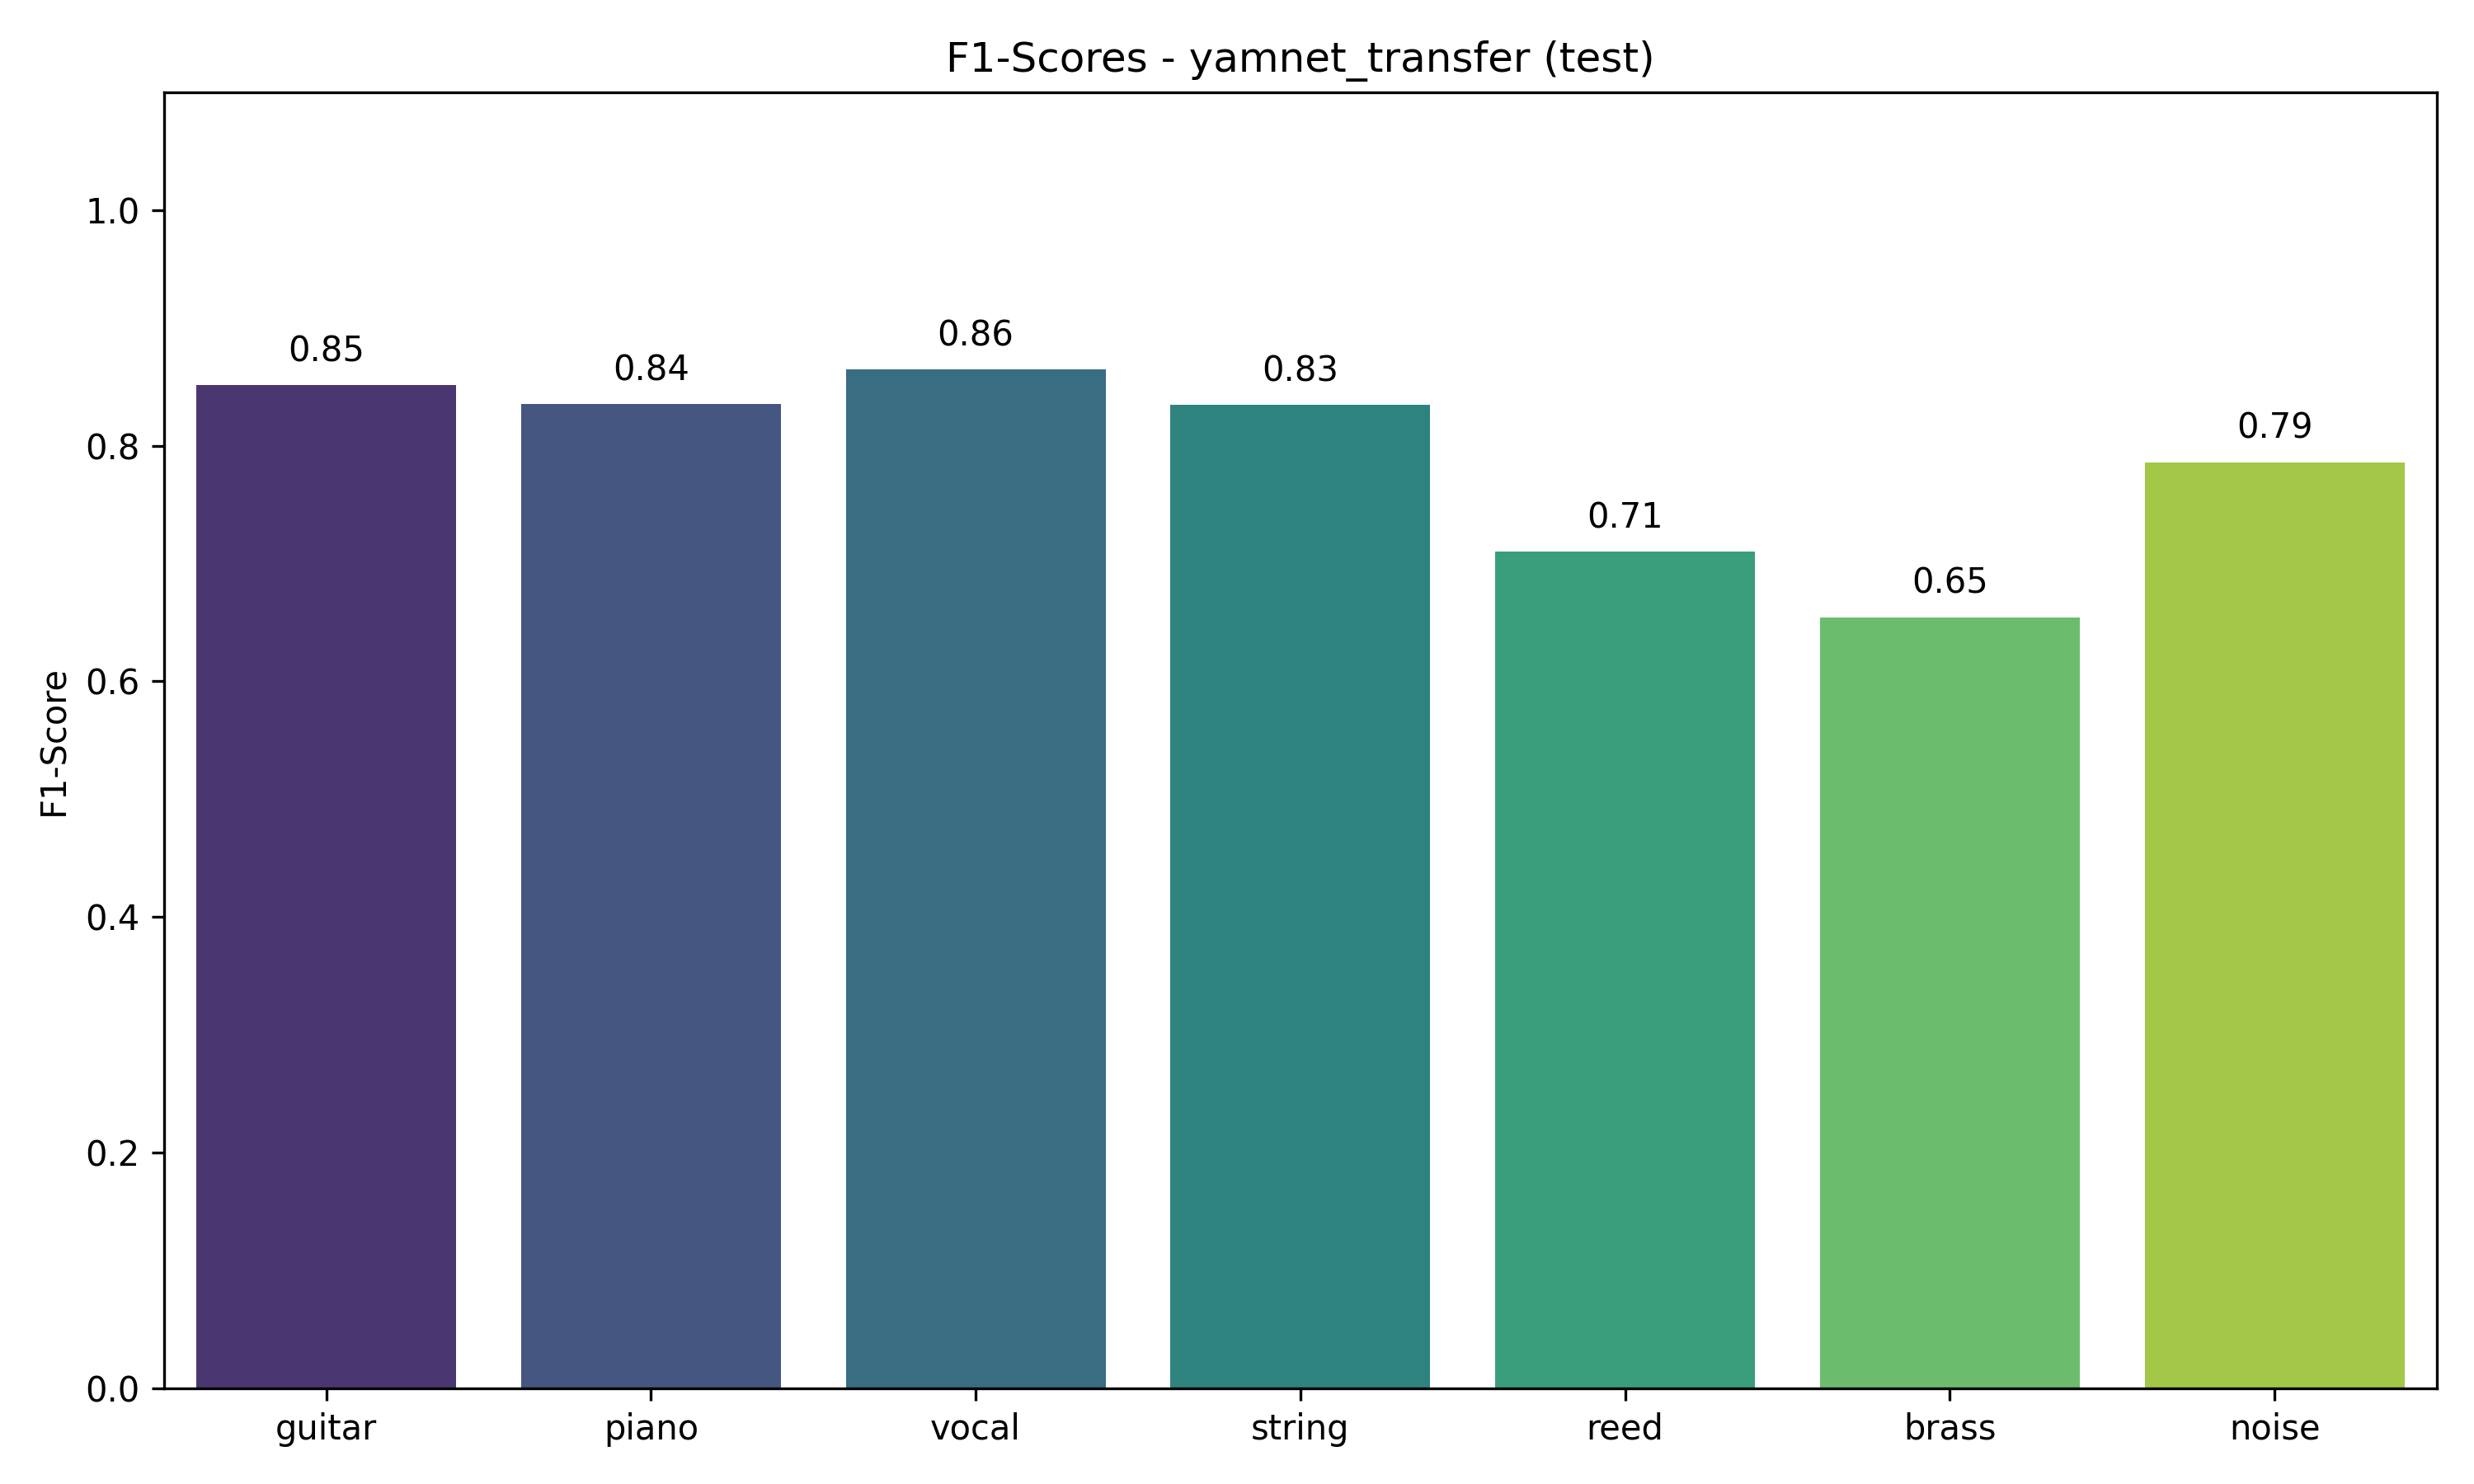
\includegraphics[width=0.82\textwidth]{fig_yamnet_test_f1_scores.png}
    \caption{A YAMNet transfer learning modell osztályonkénti F1-score értékei}
    \label{fig:yamnet_test_f1_scores}
\end{figure}

\section{A jelenlegi rendszer értékelése}
\label{sec:rendszer_ertekelese}

A mérési eredmények alapján a projekt jelenlegi állapotában nem rekordpontosságú hangszerfelismerő rendszer, hanem egy végigvezetett, működő és mérhető mérnöki megoldás. A rendszer erőssége nem abban van, hogy minden osztályban közel tökéletes eredményt ad, hanem abban, hogy a teljes út reprodukálható: az adatgyűjtéstől és szeleteléstől kezdve az augmentáción, mikrofonos újrafelvételen, jellemzőkinyerésen és tanításon át a valós idejű predikcióig.

A legfontosabb következtetések:
\begin{itemize}
    \item Az augmentáció a validációs eredmények alapján erős javító hatást mutatott.
    \item A mikrofonos környezetre való közvetlen átvitel érezhető domain shiftet okozott.
    \item A mikrofonos train adatok bevonása a célkörnyezeti teljesítményt jelentősen javította.
    \item A végső teszteredmény szerényebb, mint a legjobb validációs futás, de reálisabb képet ad a rendszer tényleges generalizációjáról.
    \item A YAMNet transfer learning erős összehasonlítási pontot adott, de a saját Log-Mel pipeline továbbra is a dolgozat fő, valós időben használt megoldása maradt.
\end{itemize}

Módszertani szempontból fontos korlát, hogy az adathalmaz mérete továbbra is viszonylag kicsi, és a saját CNN tanításai futásonként ingadoznak. Emiatt a köztes kísérletek között nem minden különbséget érdemes túl erősen értelmezni. Az viszont stabilan látszik, hogy az augmentáció és a célkörnyezeti mikrofonos adatok használata javító irányba mozdította el a rendszert. A YAMNet eredménye azt is megmutatta, hogy egy nagy, előtanított audio reprezentációval lehet még javítani a pontosságon, de a saját pipeline önmagában is működő, mérhető és valós időben használható megoldás maradt. Ez a dolgozat céljához illeszkedik: nem egy lezárt, ipari pontosságú terméket készítettem, hanem egy saját adatokon végigvezetett hangszerfelismerő rendszert, amelynek előnyei és korlátai is mérhetően megjelennek.
